\documentclass[10pt]{beamer}
\usetheme{Madrid}
\usecolortheme{default}
\usepackage[utf8]{inputenc}
\usepackage[T2A]{fontenc}
\usepackage[russian]{babel}
\usepackage{graphicx}
\usepackage{amsmath}

\title[ЕСПД и Формализация]{Стандарты ЕСПД и Формализация задачи (Вариант 5)}
\subtitle{Доклад по технологической (проектно-технологической) практике}
\author{Егоров А. В.}
\institute[МАИ]{МАИ, Кафедра 304, Группа М3О-225БВ-24}
\date{2 июля 2026 г.}

\begin{document}

\frame{\titlepage}

\begin{frame}{Содержание}
    \tableofcontents
\end{frame}

\section{ГОСТ 19.502-78: Описание применения}

\begin{frame}{ГОСТ 19.502-78. Назначение и область действия}
    \begin{itemize}
        \item \textbf{Название:} Единая система программной документации. Описание применения.
        \item \textbf{Назначение:} Устанавливает строгие требования к содержанию и оформлению программного документа <<Описание применения>>.
        \item \textbf{Область применения:} Документ предназначен исключительно для специалистов, занимающихся эксплуатацией программы. Он содержит сведения, необходимые для применения программы по ее прямому назначению.
    \end{itemize}
\end{frame}

\begin{frame}{ГОСТ 19.502-78. Состав и содержание}
    Документ должен содержать следующие основные разделы:
    \begin{enumerate}
        \item \textbf{Назначение программы:} возможности, основной алгоритм, ограничения.
        \item \textbf{Условия применения:} требования к программным и аппаратным средствам, операционной системе.
        \item \textbf{Описание задачи:} постановка задачи, формализация и методы решения.
        \item \textbf{Входные и выходные данные:} формат, организация, способы ввода/вывода.
    \end{enumerate}
\end{frame}

\section{ГОСТ 19.005-85: Схемы алгоритмов}

\begin{frame}{ГОСТ 19.005-85. Назначение}
    \begin{itemize}
        \item \textbf{Название:} ЕСПД. Схемы алгоритмов, программ, данных и систем. Условные обозначения и правила выполнения.
        \item \textbf{Суть стандарта:} Устанавливает единые условные графические обозначения для наглядного отображения логики, структуры алгоритмов и программ.
        \item \textbf{Интеграция:} Базируется на международном стандарте ISO 5807-85, обеспечивая международную совместимость технической документации.
    \end{itemize}
\end{frame}

\begin{frame}{ГОСТ 19.005-85. Требования к оформлению}
    \begin{itemize}
        \item \textbf{Линии потока:} должны быть параллельны линиям внешней рамки (строго горизонтальны или вертикальны).
        \item \textbf{Стрелки:} обязательны, если направление линии потока идет снизу вверх или справа налево.
        \item \textbf{Размеры:} ширина ($a$) и высота ($b$) символов регламентированы (рекомендовано $b = a/2$ или $b = 2a/3$, где $a$ кратно 5 мм).
    \end{itemize}
\end{frame}

\section{Формализация задачи (Вариант 5)}

\begin{frame}{Постановка задачи: Вариант 5}
    \textbf{Исследуемые векторные поля:}
    \begin{itemize}
        \item Поле $\vec{a} = y^2 \vec{i} + z^2 \vec{j} + x^2 \vec{k}$
        \item Поле $\vec{b} = (2xy^3z + y) \vec{i} + (3x^2y^2z + x) \vec{j} + (x^2y^3 + 4z^3) \vec{k}$
    \end{itemize}
    \vspace{0.5cm}
    \textbf{Область (поверхность $S$):} \\
    Часть единичной сферы $x^2 + y^2 + z^2 = 1$, расположенная в первом октанте ($x \ge 0, y \ge 0, z \ge 0$).
\end{frame}

\begin{frame}{Аналитический расчет: Поле $\vec{a}$}
    \begin{itemize}
        \item \textbf{Класс поля:} $\text{div }\vec{a} = 0$, $\text{rot }\vec{a} = -2z\vec{i} - 2x\vec{j} - 2y\vec{k} \neq 0$ \\
        $\Rightarrow$ Поле \textbf{соленоидальное}.
        \vspace{0.3cm}
        \item \textbf{Поток поля $P$:} (через поверхностный интеграл и по Гауссу-Остроградскому):
        $$ P = \iint_S \vec{a} \cdot d\vec{S} = \frac{3\pi}{16} $$
        \vspace{0.1cm}
        \item \textbf{Циркуляция $C$:} (по контуру через интеграл и по теореме Стокса):
        $$ C = \oint_L \vec{a} \cdot d\vec{r} = -2 $$
    \end{itemize}
\end{frame}

\begin{frame}{Аналитический расчет: Поле $\vec{b}$}
    \begin{itemize}
        \item \textbf{Класс поля:} $\text{rot }\vec{b} = 0$ \\
        $\Rightarrow$ Поле \textbf{потенциальное}.
        \vspace{0.3cm}
        \item \textbf{Потенциал $U(x,y,z)$:} (восстановлен по полному дифференциалу):
        $$ U(x,y,z) = xy + x^2y^3z + z^4 $$
        \vspace{0.1cm}
        \item \textbf{Работа сил поля $W$:} При перемещении материальной точки из начала координат $O(0,0,0)$ в точку $M(1,1,1)$:
        $$ W = U(1,1,1) - U(0,0,0) = 3 - 0 = 3 $$
    \end{itemize}
\end{frame}

\section{Работа с библиотечным фондом}

\begin{frame}{Подтверждение работы с первоисточниками}
    \begin{center}
        \large В рамках подготовки к докладу и выполнению проектной документации была проведена очная работа с четырехтомником стандартов ГОСТ (ЕСПД) в библиотеке МАИ (корпус 7).
    \end{center}
\end{frame}

\begin{frame}{Фото из четырехтомника}
    \begin{center}
        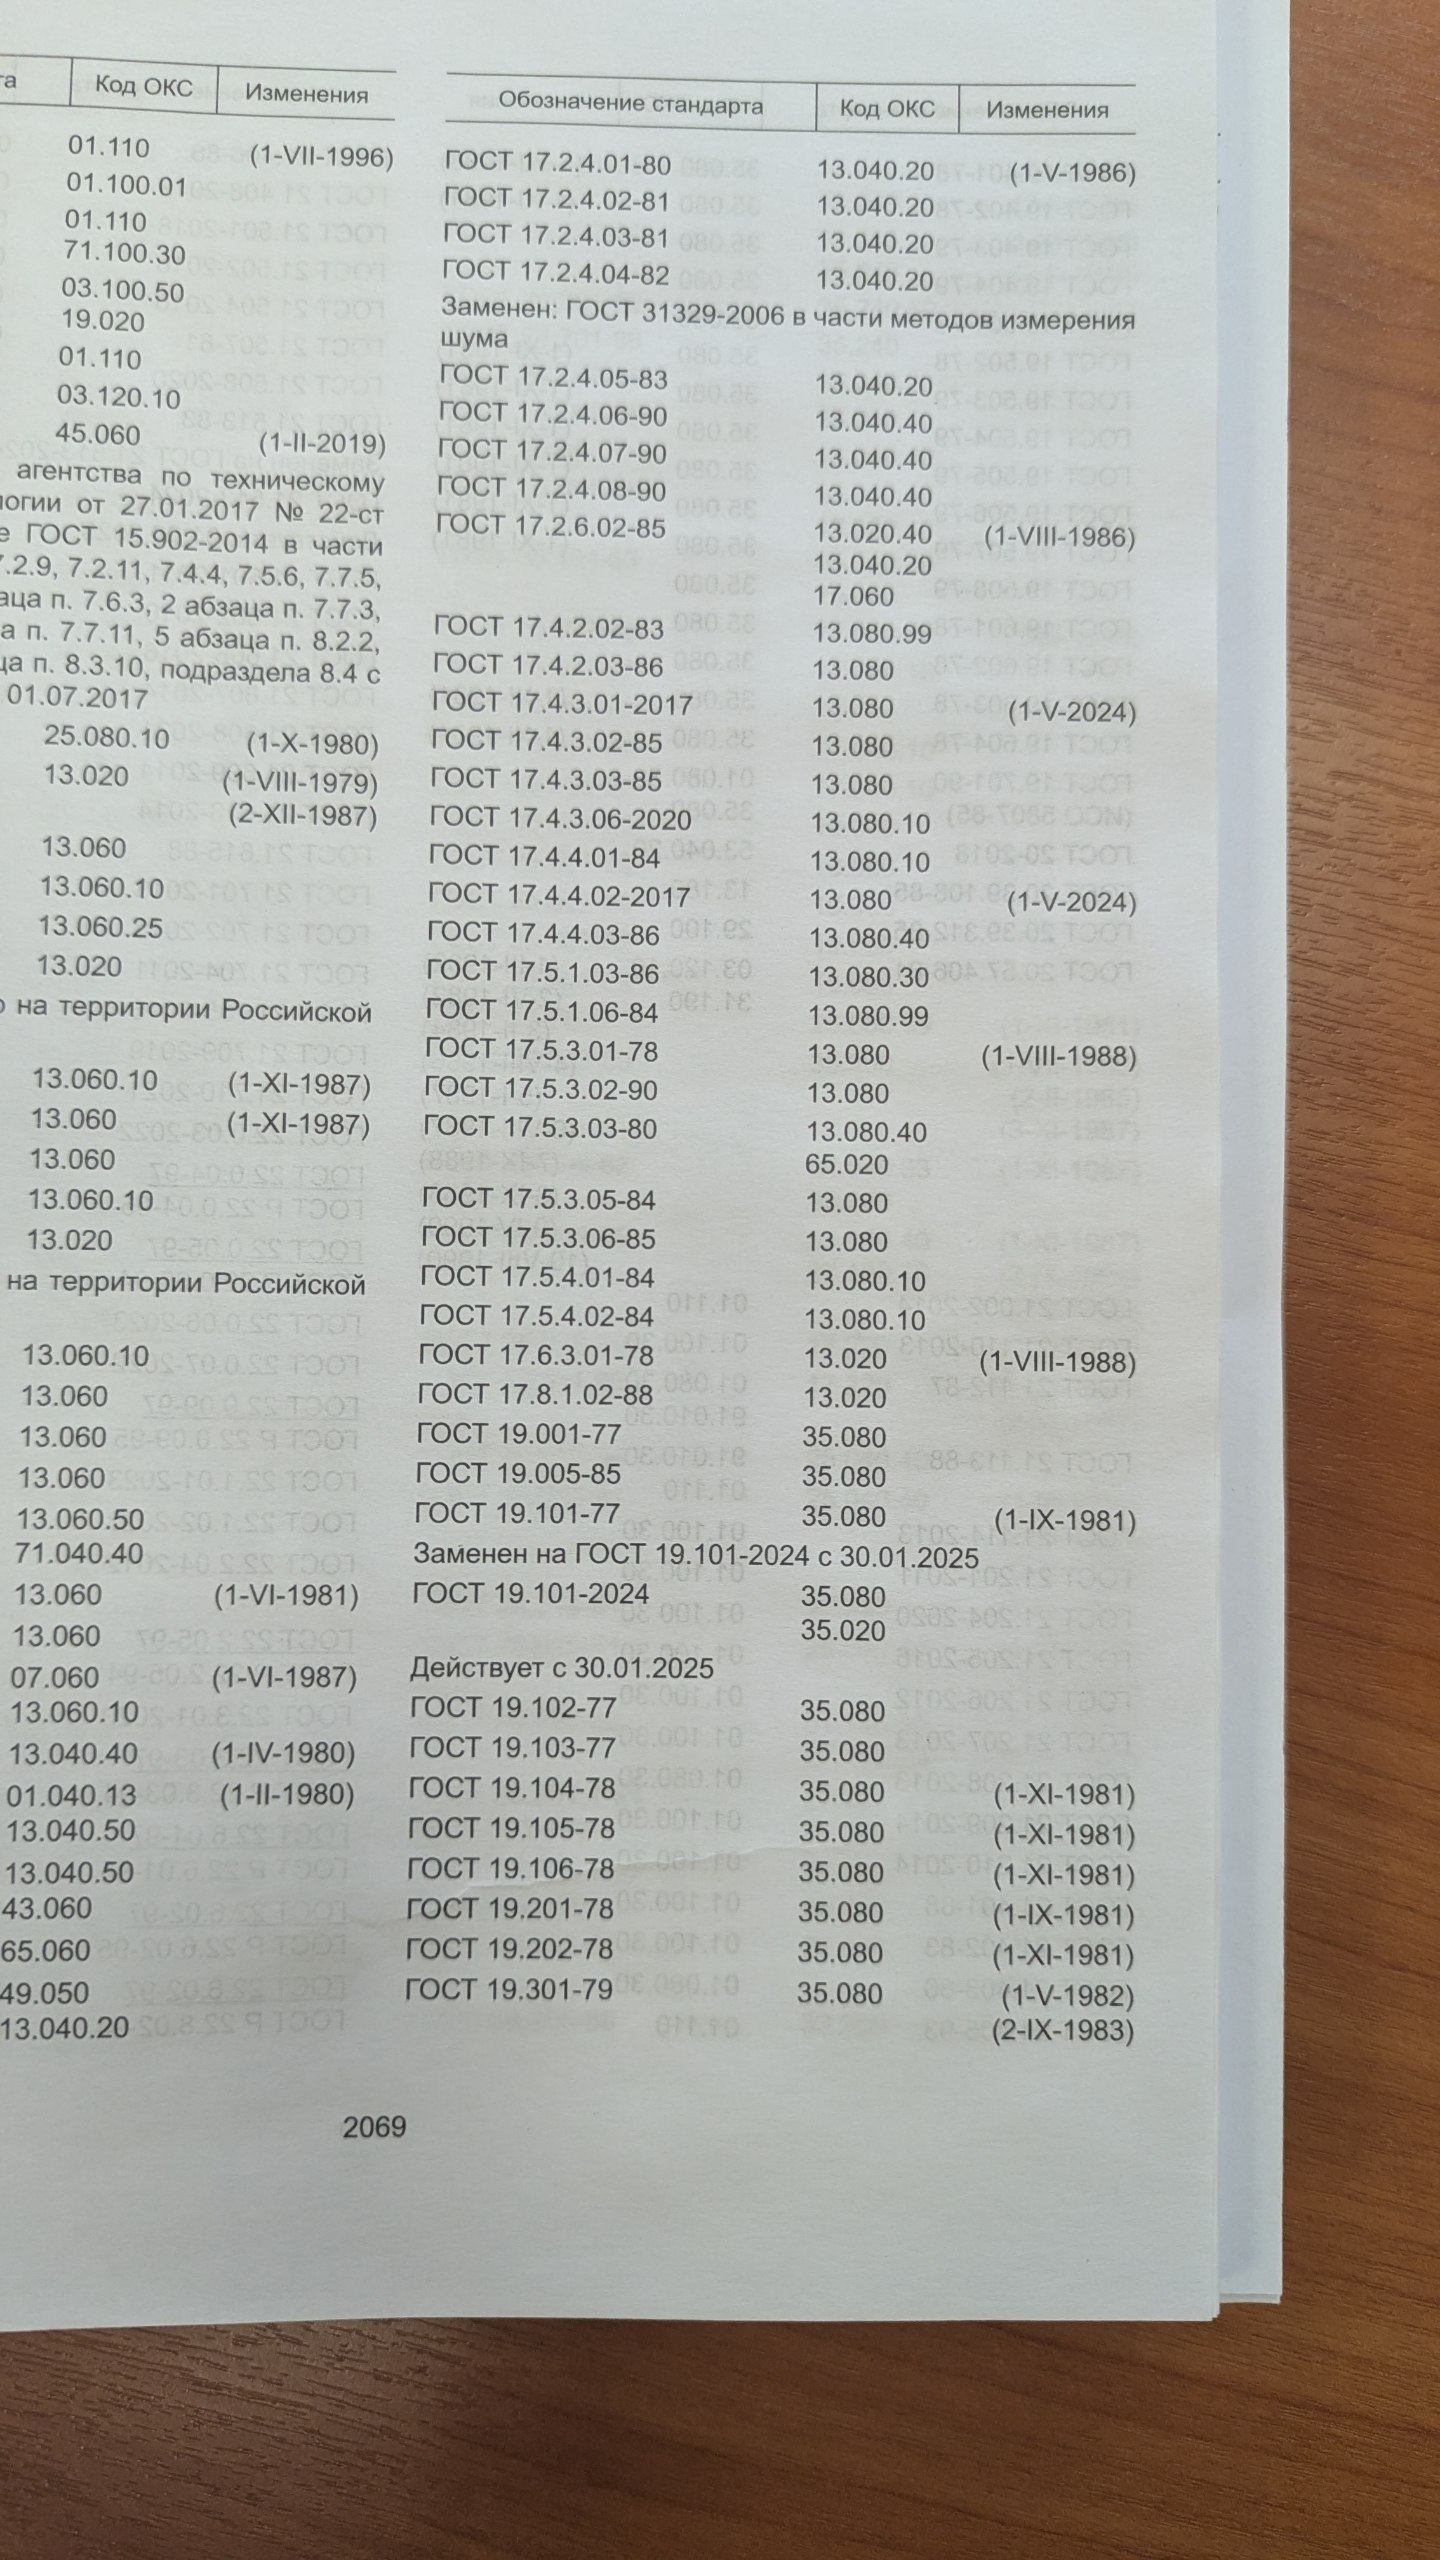
\includegraphics[width=\textwidth,height=0.75\textheight,keepaspectratio]{photo2.jpg}
    \end{center}
\end{frame}

\begin{frame}
    \begin{center}
        \Huge Спасибо за внимание! \\
        \vspace{1cm}
        \large Готов ответить на ваши вопросы.
    \end{center}
\end{frame}

\end{document}